% Options for packages loaded elsewhere
\PassOptionsToPackage{unicode}{hyperref}
\PassOptionsToPackage{hyphens}{url}
%
\documentclass[
]{book}
\usepackage{amsmath,amssymb}
\usepackage{lmodern}
\usepackage{iftex}
\ifPDFTeX
  \usepackage[T1]{fontenc}
  \usepackage[utf8]{inputenc}
  \usepackage{textcomp} % provide euro and other symbols
\else % if luatex or xetex
  \usepackage{unicode-math}
  \defaultfontfeatures{Scale=MatchLowercase}
  \defaultfontfeatures[\rmfamily]{Ligatures=TeX,Scale=1}
\fi
% Use upquote if available, for straight quotes in verbatim environments
\IfFileExists{upquote.sty}{\usepackage{upquote}}{}
\IfFileExists{microtype.sty}{% use microtype if available
  \usepackage[]{microtype}
  \UseMicrotypeSet[protrusion]{basicmath} % disable protrusion for tt fonts
}{}
\makeatletter
\@ifundefined{KOMAClassName}{% if non-KOMA class
  \IfFileExists{parskip.sty}{%
    \usepackage{parskip}
  }{% else
    \setlength{\parindent}{0pt}
    \setlength{\parskip}{6pt plus 2pt minus 1pt}}
}{% if KOMA class
  \KOMAoptions{parskip=half}}
\makeatother
\usepackage{xcolor}
\IfFileExists{xurl.sty}{\usepackage{xurl}}{} % add URL line breaks if available
\IfFileExists{bookmark.sty}{\usepackage{bookmark}}{\usepackage{hyperref}}
\hypersetup{
  pdftitle={DataScience1},
  pdfauthor={Sebastian Sauer},
  hidelinks,
  pdfcreator={LaTeX via pandoc}}
\urlstyle{same} % disable monospaced font for URLs
\usepackage{longtable,booktabs,array}
\usepackage{calc} % for calculating minipage widths
% Correct order of tables after \paragraph or \subparagraph
\usepackage{etoolbox}
\makeatletter
\patchcmd\longtable{\par}{\if@noskipsec\mbox{}\fi\par}{}{}
\makeatother
% Allow footnotes in longtable head/foot
\IfFileExists{footnotehyper.sty}{\usepackage{footnotehyper}}{\usepackage{footnote}}
\makesavenoteenv{longtable}
\usepackage{graphicx}
\makeatletter
\def\maxwidth{\ifdim\Gin@nat@width>\linewidth\linewidth\else\Gin@nat@width\fi}
\def\maxheight{\ifdim\Gin@nat@height>\textheight\textheight\else\Gin@nat@height\fi}
\makeatother
% Scale images if necessary, so that they will not overflow the page
% margins by default, and it is still possible to overwrite the defaults
% using explicit options in \includegraphics[width, height, ...]{}
\setkeys{Gin}{width=\maxwidth,height=\maxheight,keepaspectratio}
% Set default figure placement to htbp
\makeatletter
\def\fps@figure{htbp}
\makeatother
\usepackage[normalem]{ulem}
% Avoid problems with \sout in headers with hyperref
\pdfstringdefDisableCommands{\renewcommand{\sout}{}}
\setlength{\emergencystretch}{3em} % prevent overfull lines
\providecommand{\tightlist}{%
  \setlength{\itemsep}{0pt}\setlength{\parskip}{0pt}}
\setcounter{secnumdepth}{5}
\usepackage{booktabs}
\usepackage{float}
\usepackage{bm}
\usepackage{amsthm}
\makeatletter
\def\thm@space@setup{%
  \thm@preskip=8pt plus 2pt minus 4pt
  \thm@postskip=\thm@preskip
}
\makeatother
\ifLuaTeX
  \usepackage{selnolig}  % disable illegal ligatures
\fi
\usepackage[]{natbib}
\bibliographystyle{apalike}

\title{DataScience1}
\usepackage{etoolbox}
\makeatletter
\providecommand{\subtitle}[1]{% add subtitle to \maketitle
  \apptocmd{\@title}{\par {\large #1 \par}}{}{}
}
\makeatother
\subtitle{Grundlagen der Prognosemodellierung 🔮🧰}
\author{Sebastian Sauer}
\date{2022-03-10 21:21:12}

\begin{document}
\maketitle

{
\setcounter{tocdepth}{1}
\tableofcontents
}
\hypertarget{uxfcberblick}{%
\chapter{Überblick}\label{uxfcberblick}}

\begin{figure}[H]

{\centering 
\includegraphics[width=0.5\linewidth]{img/662upp} 

}

\end{figure}

\href{https://imgflip.com/i/662upp}{Imgflip Meme Generator}

\hypertarget{was-sie-hier-lernen-und-wozu-das-gut-ist}{%
\section{Was Sie hier lernen und wozu das gut ist}\label{was-sie-hier-lernen-und-wozu-das-gut-ist}}

Alle Welt spricht von Big Data, aber ohne die Analyse sind die großen Daten nur großes Rauschen. Was letztlich interessiert, sind die Erkenntnisse, die Einblicke, nicht die Daten an sich.
Dabei ist es egal, ob die Daten groß oder klein sind.
Natürlich erlauben die heutigen Datenmengen im Verbund mit leistungsfähigen Rechnern und neuen Analysemethoden ein Verständnis,
das vor Kurzem noch nicht möglich war.
Und wir stehen erst am Anfang dieser Entwicklung.
Vielleicht handelt es sich bei diesem Feld um eines der dynamischsten Fachgebiete der heutigen Zeit.
Sie sind dabei: Sie lernen einiges Handwerkszeugs des ``Datenwissenschaftlers''.
Wir konzentrieren uns auf das vielleicht bekannteste Teilgebiet:
Ereignisse vorhersagen auf Basis von hoch strukturierten Daten
und geeigneter Algorithmen und Verfahren.
Nach diesem Kurs sollten Sie in der Lage sein,
typisches Gebabbel des Fachgebiet mit Lässigkeit mitzumachen.
Ach ja, und mit einigem Erfolg Vorhersagemodelle entwickeln.

\hypertarget{lernziele}{%
\section{Lernziele}\label{lernziele}}

Nach diesem Kurs sollten Sie

\begin{itemize}
\tightlist
\item
  grundlegende Konzepte des statistischen Lernens verstehen und mit R anwenden können
\item
  gängige Prognose-Algorithmen kennen, in Grundzügen verstehen und mit R anwenden können
\item
  die Güte und Grenze von Prognosemodellen einschätzen können
\end{itemize}

\hypertarget{voraussetzungen}{%
\section{Voraussetzungen}\label{voraussetzungen}}

Um von diesem Kurs am besten zu profitieren,
sollten Sie folgendes Wissen mitbringen:

\begin{itemize}
\tightlist
\item
  grundlegende Kenntnisse im Umgang mit R, möglichst auch mit dem tidyverse
\item
  grundlegende Kenntnisse der deskriptiven Statistik
\item
  grundlegende Kenntnis der Regressionsanalyse
\end{itemize}

\hypertarget{hinweise-zu-diesem-projekt}{%
\section{Hinweise zu diesem Projekt}\label{hinweise-zu-diesem-projekt}}

\begin{itemize}
\item
  Die URL zu diesem Projekt lautet \textless test.io\textgreater.
\item
  Lesen Sie sich die folgenden Informationen bitte gut durch: \href{https://sebastiansauer.github.io/fopra/Interna/Hinweise.html}{Hinweise}
\item
  Den Quellcode finden Sie \href{https://github.com/sebastiansauer/datascience1}{in diesem Github-Repo}.
\item
  Sie haben Feedback, Fehlerhinweise oder Wünsche zur Weiterentwicklung? Am besten stellen Sie \href{https://github.com/sebastiansauer/datascience1/issues}{hier} einen \emph{Issue} ein.
\item
  Dieses Projekt steht unter der \href{https://github.com/sebastiansauer/datascience1/blob/main/LICENSE}{MIT-Lizenz}).
\end{itemize}

\hypertarget{lernhilfen}{%
\section{Lernhilfen}\label{lernhilfen}}

\hypertarget{software}{%
\subsection{Software}\label{software}}

\begin{itemize}
\tightlist
\item
  Installieren Sie \href{https://data-se.netlify.app/2021/11/30/installation-von-r-und-seiner-freunde/}{R und seine Freunde}.
\item
  Installieren Sie die folgende R-Pakete:

  \begin{itemize}
  \tightlist
  \item
    tidyverse
  \item
    tidymodels
  \item
    weitere Pakete werden im Unterricht bekannt gegeben (es schadet aber nichts, jetzt schon Pakete nach eigenem Ermessen zu installieren)
  \end{itemize}
\item
  \href{https://github.com/sebastiansauer/Lehre}{R Syntax aus dem Unterricht} findet sich im Github-Repo bzw. Ordner zum jeweiligen Semester.
\end{itemize}

\hypertarget{online-zusammenarbeit}{%
\subsection{Online-Zusammenarbeit}\label{online-zusammenarbeit}}

\begin{itemize}
\tightlist
\item
  \href{https://frag.jetzt/home}{Frag-Jetzt-Raum zum anonymen Fragen stellen während des Unterrichts}. Der Keycode wird Ihnen vom Dozenten bereitgestellt.
\item
  \href{https://de.padlet.com/}{Padlet} zum einfachen (und anonymen) Hochladen von Arbeitsergebnissen der Studentis im Unterricht. Wir nutzen es als eine Art Pinwand zum Sammeln von Arbeitsbeiträgen. Die Zugangsdaten stellt Ihnen der Dozent bereit.
\end{itemize}

\hypertarget{modulzeitplan}{%
\section{Modulzeitplan}\label{modulzeitplan}}

\begin{longtable}[]{@{}llll@{}}
\toprule
Nr. & Kalenderwoche & Datum & Thema \\
\midrule
\endhead
1 & 11 & 14.-18.3.22 & Grundkonzepte \\
2 & 12 & 21.3.-25.3. & tidyverse, 2. Blick \\
3 & 13 & 28.3.-1.4. & tidymodels \\
4 & 14 & 4.4.-8.4. & kNN \\
5 & 15 & 11.4.-15.4. & Statistisches Lernen \\
6 & 16 & 18.4.-22.4 & Wiederholung \\
7 & 17 & 25.4.-29.4 & Logistische Regression \\
8 & 18 & 2.5.-6.5. & Naive Bayes \\
9 & 19 & 9.5.-13.5. & Entscheidungsbäume \\
10 & 20 & 16.5.-20.5. & Zufallswälder \\
11 & 21 & 23.5.-27.5. & Fallstudie \\
12 & 23 & 6.6.-10.6. & Wiederholung \\
13 & 24 & 13.6.-17.6. & GAM \\
14 & 25 & 20.6.-24.6. & Lasso und Co \\
15 & 26 & 27.6.-1.7. & Vertiefung \\
\bottomrule
\end{longtable}

\hypertarget{literatur}{%
\section{Literatur}\label{literatur}}

Zentrale Kursliteratur für die theoretischen Konzepte ist \citep{rhys}.
Die praktische Umsetzung in R basiert auf \citep{silge_tidy_2022}. Eine theoretische Konzepte sind \citet{james_introduction_2021} entnommen.

\hypertarget{faq}{%
\section{FAQ}\label{faq}}

\begin{itemize}
\tightlist
\item
  \emph{Folien}

  \begin{itemize}
  \tightlist
  \item
    Frage: Gibt es ein Folienskript?
  \item
    Antwort: Wo es einfache, gute Literatur gibt, gibt es kein Skript. Wo es keine gute oder keine einfach zugängliche Literatur gibt, dort gibt es ein Skript.
  \end{itemize}
\item
  \emph{Englisch}

  \begin{itemize}
  \tightlist
  \item
    Ist die Literatur auf Englisch?
  \item
    Ja. Allerdings ist die Literatur gut zugänglich. Das Englisch ist nicht schwer. Bedenken Sie: Englisch ist die lingua franca in Wissenschaft und Wirtschaft. Ein solides Verständnis englischer (geschriebener) Sprache ist für eine gute Ausbildung unerlässlich. Zu dem sollte die Kursliteratur fachlich passende und gute Bücher umfassen; oft sind das englische Titel.
  \end{itemize}
\item
  \emph{Anstrengend}

  \begin{itemize}
  \tightlist
  \item
    Ist der Kurs sehr anstrengend, aufwändig?
  \item
    Der Kurs hat ein mittleres Anspruchsniveau.
  \end{itemize}
\item
  \emph{Mathe}

  \begin{itemize}
  \tightlist
  \item
    Muss man ein Mathe-Crack sein, um eine gute Note zu erreichen?
  \item
    Nein. Mathe steht nicht im Vordergrund. Schauen Sie sich die Literatur an, sie werden wenig Mathe darin finden.
  \end{itemize}
\item
  \emph{Prüfungsliteratur}

  \begin{itemize}
  \tightlist
  \item
    Welche Literatur ist prüfungsrelevant?
  \item
    Die Prüfung ist angewandt, z.B. ein Prognosewettbewerb. Es wird keine Klausur geben, in der reines Wissen abgefragt wird.
  \end{itemize}
\item
  \emph{Nur R?}

  \begin{itemize}
  \tightlist
  \item
    Wird nur R in dem Kurs gelehrt? Andere Programmiersprachen sind doch auch wichtig.
  \item
    In der Datenanalyse gibt es zwei zentrale Programmiersprachen, R und Python. Beide sind gut und beide werden viel verwendet. In einer Grundausbildung sollte man sich auf eine Sprache begrenzen, da sonst den Sprachen zu viel Zeit eingeräumt werden muss. Wichtiger als eine zweite Programmiersprache zu lernen, mit der man nicht viel mehr kann als mit der ersten, ist es, die Inhalte des Fachs zu lernen.
  \end{itemize}
\end{itemize}

\hypertarget{moduluxfcberblick}{%
\chapter{Modulüberblick}\label{moduluxfcberblick}}

\hypertarget{grundkonzepte}{%
\section{Grundkonzepte}\label{grundkonzepte}}

\hypertarget{datum}{%
\subsection{Datum}\label{datum}}

\begin{itemize}
\tightlist
\item
  14.-18.3.22
\end{itemize}

\hypertarget{lernziele-1}{%
\subsection{Lernziele}\label{lernziele-1}}

\begin{itemize}
\tightlist
\item
  Sie können erläutern, was man unter statistischem Lernen versteht.
\item
  Sie wissen, war Overfitting ist, wie es entsteht, und wie es vermieden werden kann.
\item
  Sie kennen verschiedenen Arten von statistischem Lernen und können Algorithmen zu diesen Arten zuordnen.
\end{itemize}

\hypertarget{vorbereitung}{%
\subsection{Vorbereitung}\label{vorbereitung}}

\begin{itemize}
\tightlist
\item
  Lesen Sie die Hinweise zum Modul.
\item
  Installieren (oder Updaten) Sie die für dieses Modul angegeben Software.
\item
  Lesen Sie die Literatur.
\end{itemize}

\hypertarget{literatur-1}{%
\subsection{Literatur}\label{literatur-1}}

\begin{itemize}
\tightlist
\item
  Rhys, Kap. 1
\end{itemize}

\hypertarget{skript}{%
\subsection{Skript}\label{skript}}

\begin{itemize}
\tightlist
\item
  \href{}{Kap. 1}
\end{itemize}

\hypertarget{aufgaben}{%
\subsection{Aufgaben}\label{aufgaben}}

\begin{itemize}
\tightlist
\item
  \href{https://www.kaggle.com/}{Machen Sie sich mit `Kaggle' vertraut}
\item
  \href{https://www.kaggle.com/pranjalpandey12/performing-simple-linear-regression-in-r}{Arbeiten Sie diese Regressionsfallstudie (zum Thema Gehalt) auf Kaggle auf}
\item
  \href{https://www.kaggle.com/lazaro97/data-preprocessing-and-linear-regression-with-r}{Werfen Sie einen Blick in diese Fallstudie auf Kaggle zum Thema Hauspreise}
\item
  \href{https://data-se.netlify.app/2021/03/10/fallstudie-modellierung-von-flugversp\%C3\%A4tungen/}{Wiederholen Sie unser Vorgehen in der Fallstudie zu den Flugverspätungen}
\end{itemize}

\hypertarget{vertiefung}{%
\subsection{Vertiefung}\label{vertiefung}}

\begin{itemize}
\tightlist
\item
  \href{https://www.zeit.de/arbeit/2020-10/data-scientist-gehalt-geldanlage-programmieren-kontoauszug}{Verdienst einer deutschen Data Scientistin}
\item
  \href{https://www.kaggle.com/micahshull/r-bike-sharing-linear-regression}{Weitere Fallstudie zum Thema Regression auf Kaggle}
\item
  \href{https://www.coursera.org/learn/data-science-course}{Crashkurs Data Science (Coursera, Johns Hopkins University) mit `Star-Dozenten'}
\end{itemize}

\hypertarget{hinweise}{%
\subsection{Hinweise}\label{hinweise}}

\begin{itemize}
\tightlist
\item
  Bitte beachten Sie die Hinweise zum Präsenzunterricht und der Streamingoption.
\item
  Bitte stellen Sie sicher, dass Sie einen einsatzbereiten Computer haben und dass die angegebene Software (in aktueller Version) läuft.
\end{itemize}

\hypertarget{tidyverse-2.-blick}{%
\section{tidyverse, 2. Blick}\label{tidyverse-2.-blick}}

\hypertarget{datum-1}{%
\subsection{Datum}\label{datum-1}}

\begin{itemize}
\tightlist
\item
  21.3.-25.3.
\end{itemize}

\hypertarget{lernziele-2}{%
\subsection{Lernziele}\label{lernziele-2}}

\begin{itemize}
\tightlist
\item
  Sie können Funktionen, auch anonyme, in R schreiben.
\item
  Sie können Datensätze vom Lang- und Breit-Format wechseln.
\item
  Sie können Mapping-Funktionen anwenden.
\item
  Sie können eine dplyr-Funktion auf mehrere Spalten gleichzeitig anwenden.
\end{itemize}

\hypertarget{vorbereitung-1}{%
\subsection{Vorbereitung}\label{vorbereitung-1}}

\begin{itemize}
\tightlist
\item
  Lesen Sie die Literatur.
\end{itemize}

\hypertarget{literatur-2}{%
\subsection{Literatur}\label{literatur-2}}

\begin{itemize}
\tightlist
\item
  Rhys, Kap. 2
\end{itemize}

\hypertarget{tidymodels}{%
\section{tidymodels}\label{tidymodels}}

\hypertarget{datum-2}{%
\subsection{Datum}\label{datum-2}}

\begin{itemize}
\tightlist
\item
  28.3.-1.4.
\end{itemize}

\hypertarget{literatur-3}{%
\subsection{Literatur}\label{literatur-3}}

\begin{itemize}
\tightlist
\item
  TMWR
\end{itemize}

\hypertarget{knn}{%
\section{kNN}\label{knn}}

\hypertarget{datum-3}{%
\subsection{Datum}\label{datum-3}}

\begin{itemize}
\tightlist
\item
  4.4.-8.4.
\end{itemize}

\hypertarget{literatur-4}{%
\subsection{Literatur}\label{literatur-4}}

\begin{itemize}
\tightlist
\item
  Rhys, Kap. 3
\end{itemize}

\hypertarget{statistisches-lernen}{%
\section{Statistisches Lernen}\label{statistisches-lernen}}

\hypertarget{datum-4}{%
\subsection{Datum}\label{datum-4}}

\begin{itemize}
\tightlist
\item
  11.4.-15.4.
\end{itemize}

\hypertarget{literatur-5}{%
\subsection{Literatur}\label{literatur-5}}

\begin{itemize}
\tightlist
\item
  Rhys, Kap. 3
\end{itemize}

\hypertarget{vertiefung-1}{%
\subsection{Vertiefung}\label{vertiefung-1}}

\begin{itemize}
\tightlist
\item
  \href{https://xkcd.com/435/}{Fields arranged by purity, xkcd 435}
\end{itemize}

\hypertarget{hinweise-1}{%
\subsection{Hinweise}\label{hinweise-1}}

\begin{itemize}
\tightlist
\item
  In dieser Woche fällt die Übung aus (Ostern).
\end{itemize}

\hypertarget{wiederholung}{%
\section{Wiederholung}\label{wiederholung}}

\hypertarget{datum-5}{%
\subsection{Datum}\label{datum-5}}

\begin{itemize}
\tightlist
\item
  18.4.-22.4
\end{itemize}

\hypertarget{hinweise-2}{%
\subsection{Hinweise}\label{hinweise-2}}

\begin{itemize}
\tightlist
\item
  In dieser Woche fällt die Vorlesung aus (Ostern).
\end{itemize}

\hypertarget{logistische-regression}{%
\section{Logistische Regression}\label{logistische-regression}}

\hypertarget{datum-6}{%
\subsection{Datum}\label{datum-6}}

\begin{itemize}
\tightlist
\item
  25.4.-29.4
\end{itemize}

\hypertarget{literatur-6}{%
\subsection{Literatur}\label{literatur-6}}

\begin{itemize}
\tightlist
\item
  Rhys, Kap. 4
\end{itemize}

\hypertarget{naive-bayes}{%
\section{Naive Bayes}\label{naive-bayes}}

\hypertarget{datum-7}{%
\subsection{Datum}\label{datum-7}}

\begin{itemize}
\tightlist
\item
  2.5.-6.5.
\end{itemize}

\hypertarget{literatur-7}{%
\subsection{Literatur}\label{literatur-7}}

\begin{itemize}
\tightlist
\item
  Rhys, Kap. 6
\end{itemize}

\hypertarget{entscheidungsbuxe4ume}{%
\section{Entscheidungsbäume}\label{entscheidungsbuxe4ume}}

\hypertarget{datum-8}{%
\subsection{Datum}\label{datum-8}}

\begin{itemize}
\tightlist
\item
  9.5.-13.5.
\end{itemize}

\hypertarget{literatur-8}{%
\subsection{Literatur}\label{literatur-8}}

\begin{itemize}
\tightlist
\item
  Rhys, Kap. 7
\end{itemize}

\hypertarget{zufallswuxe4lder}{%
\section{Zufallswälder}\label{zufallswuxe4lder}}

\hypertarget{datum-9}{%
\subsection{Datum}\label{datum-9}}

\begin{itemize}
\tightlist
\item
  16.5.-20.5.
\end{itemize}

\hypertarget{literatur-9}{%
\subsection{Literatur}\label{literatur-9}}

\begin{itemize}
\tightlist
\item
  Rhys, Kap. 8
\end{itemize}

\hypertarget{fallstudie}{%
\section{Fallstudie}\label{fallstudie}}

\hypertarget{datum-10}{%
\subsection{Datum}\label{datum-10}}

\begin{itemize}
\tightlist
\item
  23.5.-27.5.
\end{itemize}

\hypertarget{literatur-10}{%
\subsection{Literatur}\label{literatur-10}}

\begin{itemize}
\tightlist
\item
  Rhys, Kap.9
\end{itemize}

\hypertarget{hinweise-3}{%
\subsection{Hinweise}\label{hinweise-3}}

\begin{itemize}
\tightlist
\item
  Nächste Woche ist Blockwoche; es findet kein regulärer Unterricht statt.
\item
  Diese Woche fällt die Übung aus.
\end{itemize}

\hypertarget{wiederholung-1}{%
\section{Wiederholung}\label{wiederholung-1}}

\hypertarget{datum-11}{%
\subsection{Datum}\label{datum-11}}

\begin{itemize}
\tightlist
\item
  6.6.-10.6.
\end{itemize}

\hypertarget{hinweise-4}{%
\subsection{Hinweise}\label{hinweise-4}}

\begin{itemize}
\tightlist
\item
  In dieser Woche fällt die Vorlesung aus (Pfingsten).
\end{itemize}

\hypertarget{gam}{%
\section{GAM}\label{gam}}

\hypertarget{datum-12}{%
\subsection{Datum}\label{datum-12}}

\begin{itemize}
\tightlist
\item
  13.6.-17.6.
\end{itemize}

\hypertarget{literatur-11}{%
\subsection{Literatur}\label{literatur-11}}

\begin{itemize}
\tightlist
\item
  Rhys, Kap. 10
\end{itemize}

\hypertarget{lasso-und-co}{%
\section{Lasso und Co}\label{lasso-und-co}}

\hypertarget{datum-13}{%
\subsection{Datum}\label{datum-13}}

\begin{itemize}
\tightlist
\item
  20.6.-24.6.
\end{itemize}

\hypertarget{literatur-12}{%
\subsection{Literatur}\label{literatur-12}}

\begin{itemize}
\tightlist
\item
  Rhys, Kap. 11
\end{itemize}

\hypertarget{vertiefung-2}{%
\section{Vertiefung}\label{vertiefung-2}}

\hypertarget{datum-14}{%
\subsection{Datum}\label{datum-14}}

\begin{itemize}
\tightlist
\item
  27.6.-1.7.
\end{itemize}

\hypertarget{literatur-13}{%
\subsection{Literatur}\label{literatur-13}}

\begin{itemize}
\tightlist
\item
  Rhys, Kap. 12
\end{itemize}

\hypertarget{vertiefung-3}{%
\subsection{Vertiefung}\label{vertiefung-3}}

\begin{itemize}
\tightlist
\item
  \href{https://medium.com/swlh/how-to-structure-a-python-based-data-science-project-a-short-tutorial-for-beginners-7e00bff14f56}{Wie man eine Data-Science-Projekt strukturiert}
\end{itemize}

\hypertarget{hinweise-5}{%
\subsection{Hinweise}\label{hinweise-5}}

\begin{itemize}
\tightlist
\item
  Nach dieser Woche endet der Unterricht.
\end{itemize}

\hypertarget{pruxfcfung}{%
\chapter{Prüfung}\label{pruxfcfung}}

\hypertarget{tldr-zusammenfassung}{%
\section{tl;dr: Zusammenfassung}\label{tldr-zusammenfassung}}

Vorhersagen sind eine praktische Sache, zumindest wenn Sie stimmen.
Wenn Sie den DAX-Stand von morgen genau vorhersagen können,
rufen Sie mich bitte sofort an. Genau das ist Ihre Aufgabe in dieser Prüfungsleistung:
Sie sollen Werte vorhersagen.

Etwas konkreter: Stellen Sie sich ein paar Studentis vor.
Von allen wissen Sie, wie lange die Person für die Statistikklausur gelernt hat.
Außerdem wissen Sie die Motivation jeder Person und vielleicht noch ein paar noten-relevante Infos.
Und Sie wissen die Note jeder Person in der Statistikklausur.
Auf dieser Basis fragt sie ein Student (Alois), der im kommenden Semester die Prüfung in Statistik schreiben \sout{muss} will:
``Sag mal, wenn ich 100 Stunden lerne und so mittel motiviert bin (bestenfalls), welche Note kann ich dann erwarten?''.
Mit Hilfe Ihrer Analyse können Sie diese Frage (und andere) beantworten.
Natürlich könnten Sie es sich leicht machen und antworten:
``Mei, der Notendurchschnitt war beim letzten Mal 2.7.
Also ist 2.7 kein ganz doofer Tipp für deine Note.''
Ja, das ist keine doofe Antwort, aber man genauere Prognose machen,
wenn man es geschickt anstellt.
Da hilft Ihnen die Statistik (doch, wirklich).

Kurz gesagt gehen Sie so vor:
Importieren Sie die Daten in R, starten Sie die nötigen R-Pakete und
schauen Sie sich die Daten unter verschiedenen Blickwinkeln an.
Dann nehmen Sie die vielversprechendsten Prädiktoren in ein Regressionsmodell und schauen sich an,
wie gut die Vorhersage ist.
Wiederholen Sie das ein paar Mal, bis Sie ein Modell haben, das Sie brauchbar finden.
Mit diesem Modell sagen Sie dann die Noten der neuen Studis (Alois und Co.) vorher.
Je genauer Ihre Vorhersage, desto besser ist Ihr Prüfungsergebnis.

\hypertarget{vorhersage}{%
\section{Vorhersage}\label{vorhersage}}

Neben der erklärenden, rückwärtsgerichteten Modellierung spielt insbesondere in der Praxis die \emph{vorhersageorientierte} Modellierung eine wichtige Rolle:
Ziel ist es, bei gegebenen, neuen Beobachtungen die noch unbekannten Werte der Zielvariablen \(y\) \emph{vorherzusagen}, z.B. für neue Kunden auf Basis von soziodemographischen Daten den \emph{Kundenwert} -- möglichst genau -- zu prognostizieren.
Dies geschieht auf Basis der vorhandenen Daten der Bestandskunden,
d.h. inklusive des für diese Kunden bekannten Kundenwertes.

Ihnen werden \emph{zwei Teildatenmengen} zur Verfügung gestellt:
Zum einen gibt es die Trainingsdaten (auch \emph{Lerndaten} genannt) und zum anderen gibt es Anwendungsdaten (auch \emph{Testdaten} genannt), auf die man das Modell anwendet.

\begin{enumerate}
\def\labelenumi{\arabic{enumi}.}
\item
  Bei den Trainingsdaten (Train-Sample) liegen sowohl die erklärenden Variablen \({\bf{x}} = (x_1, x_2, \ldots, x_n)\) als auch die Zielvariable \(y\) vor.
  Auf diesen Trainingsdaten wird das Modell \(y=f({x})+\epsilon = f(x_1, x_2, \ldots, x_n)+\epsilon\) gebildet und durch \(\hat{f}(\cdot)\) geschätzt. Es ist also die Variable \(y\) vorherszusagen.
\item
  Dieses geschätzte Modell (\(\hat{f}(\cdot)\)) wird auf die Anwendungsdaten \(\bf{x}_0\), für die (Ihnen) die Werte der Zielvariable \(y\) unbekannt sind, angewendet, d.h., es wird \(\hat{y}_0 :=\hat{f}({\bf{x}}_0)\) berechnet.
  Der unbekannte Wert \(y_0\) der Zielvariable \(y\) wird durch \(\hat{y}_0\) prognostiziert.
\end{enumerate}

Liegt zu einem noch späteren Zeitpunkt der eingetroffene Wert \(y_0\) der Zielvariable \(y\) vor, so kann die eigene Vorhersage \(\hat{y}_0\) evaluiert werden,
d.h. z.B. kann der Fehler \(e=y_0-\hat{y}_0\) zwischen prognostiziertem Wert \(\hat{y}_0\) und wahrem Wert \(y_0\) analysiert werden.

In der praktischen Anwendung können zeitlich drei aufeinanderfolgende Schritte unterschieden werden (vergleiche oben):

\begin{enumerate}
\def\labelenumi{\arabic{enumi}.}
\item
  die \emph{Trainingsphase}, d.h., die Phase für die sowohl erklärende (\({\bf{x}}\)) als auch die erklärte Variable (\(y\)) bekannt sind. Hier wird das Modell geschätzt (gelernt): \(\hat{f}(\bf{x})\). Dafür wird der Trainingsdatensatz genutzt.
\item
  In der folgenden \emph{Anwendungsphase} sind nur die erklärenden Variablen (\({\bf{x_0}}\)) bekannt, nicht \(y_0\). Auf Basis der Ergebnisses aus dem 1. Schritt wird \(\hat{y}_0 :=\hat{f}({\bf{x}}_0)\) prognostiziert.
\item
  Evt. gibt es später noch die \emph{Evaluierungsphase}, für die dann auch die Zielvariable (\(y_0\)) bekannt ist, so dass die Vorhersagegüte des Modells überprüft werden kann.
\end{enumerate}

Im Computer kann man dieses Anwendungsszenario \emph{simulieren}:
man teilt die Datenmenge \emph{zufällig} in eine Lern- bzw. Trainingsstichprobe (Trainingsdaten; \((\bf{x},y)\)) und eine Teststichprobe (Anwendungsdaten, \((\bf{x_0})\)) auf:
Die Modellierung erfolgt auf den Trainingsdaten.
Das Modell wird angewendet auf die Testdaten (Anwendungsdaten).
Da man hier aber auch die Zielvariable (\(y_0\)) kennt, kann damit das Modell evaluiert werden.

\hypertarget{hauptziel-genaue-prognose}{%
\section{Hauptziel: Genaue Prognose}\label{hauptziel-genaue-prognose}}

Ihre Aufgabe ist: Spielen Sie den Data-Scientist!
Konstruieren Sie ein Modell auf Basis der Trainingsdaten \((\bf{x},y\))
und sagen Sie für die Anwendungsdaten (\(\bf{x_0}\)) die Zielvariable möglichst genau voraus (\(\hat{y}_0\)).

Ihr(e) Dozent*in kennt den Wert der Zielvariable (\(y_0\)).

Von zwei Prognosemodellen zum gleichen Datensatz ist dasjenige Modell besser,
das weniger Vorhersagefehler aufweist, also genauer vorhersagt.
Kurz gesagt: Genauer ist besser.

\hypertarget{zum-aufbau-ihrer-prognosedatei-im-csv-format}{%
\section{Zum Aufbau Ihrer Prognosedatei im CSV-Format}\label{zum-aufbau-ihrer-prognosedatei-im-csv-format}}

\begin{enumerate}
\def\labelenumi{\arabic{enumi}.}
\tightlist
\item
  Die CSV-Datei muss aus genau zwei Spalten mit (exakt) folgenden Spaltennamen bestehen:
\end{enumerate}

\begin{enumerate}
\def\labelenumi{\alph{enumi})}
\tightlist
\item
  \texttt{id}: Den ID-Wert jedes vorhergesagten Wertes
\item
  \texttt{pred}: Der vorhergesagte Wert.
\end{enumerate}

\begin{enumerate}
\def\labelenumi{\arabic{enumi}.}
\setcounter{enumi}{2}
\item
  Umlaute sind zu ersetzen (also \texttt{Süß} wird \texttt{Suess} etc.).
\item
  Die CSV-Datei muss als \emph{Spaltentrennzeichen} ein \emph{Komma} verwenden und als \emph{Dezimaltrennzeichen} einen \emph{Punkt} (d.h. also die \emph{Standardformatierung} einer CSV-Datei; \emph{nicht} die deutsche Formatierung).
\item
  Die CSV-Datei muss genau die Anzahl an Zeilen aufweisen, die der Zeilenlänge im Test-Datensatz entspricht.
\item
  Prüfen Sie, dass Ihre CSV-Datei sich problemlos lesen lässt.
  Falls keine (funktionstüchtige) CSV-Datei eingereicht (hochgeladen) wurde, ist die Prüfung nicht bestanden.
  Tipp: Öffnen Sie die CSV-Datei mit einem Texteditor und schauen Sie sich an, ob alles vernünftig aussieht.
  Achtung: Öffnen Sie die CSV-Datei besser nicht mit Excel, da Excel einen Bug hat,
  der CSV-Dateien verfälschen kann auch ohne dass man die Datei speichert.
\end{enumerate}

\hypertarget{einzureichende-dateien}{%
\section{Einzureichende Dateien}\label{einzureichende-dateien}}

\begin{enumerate}
\def\labelenumi{\arabic{enumi}.}
\item
  Folgende* Dateiarten* sind einzureichen:

  \begin{enumerate}
  \def\labelenumii{\arabic{enumii}.}
  \tightlist
  \item
    Prognose: Ihre \emph{Prognose-Datei} (CSV-Datei)
  \item
    Analyse: Ihr \emph{Analyseskript} (R-, Rmd- oder Rmd-Notebook-Datei)
  \end{enumerate}
\item
  Weitere Dateien sind nicht einzureichen.
\item
  Komprimieren Sie die Dateien \emph{nicht} (z.B. via \emph{zip}).
\item
  Der Name jeder eingereichnte Datei muss wie folgt lauten: \texttt{Nachname\_Vorname\_Matrikelnummer\_Dateiart.Endung}. Beispiel: \texttt{Sauer\_Sebastian\_0123456\_Prognose.csv} bzw. \texttt{Sauer\_Sebastian\_0123456\_Analyse.Rmd}.
\end{enumerate}

\hypertarget{tipps}{%
\section{Tipps}\label{tipps}}

\hypertarget{tipps-fuxfcr-eine-gute-prognose}{%
\subsection{Tipps für eine gute Prognose}\label{tipps-fuxfcr-eine-gute-prognose}}

\begin{itemize}
\item
  Schauen Sie in die Literatur.
\item
  Evtl. kann eine Datenvorverarbeitung (Variablentransformation, z.B. \(\log()\) oder die Elimination von Ausreißern) helfen.
\item
  Überlegen Sie sich Kriterien zur Modell- und/ oder Variablenauswahl. Auch hierfür gibt es Algorithmen und R-Funktionen.
\item
  Vermeiden Sie Über-Anpassung (Overfitting).
\item
  Vermeiden Sie viele fehlende Werte bei Ihrer Prognose. Fehlende Werte werden bei der Benotung mit dem Mittelwert (der vorhandenen Prognosewerte Ihrer Einreichung) aufgefüllt.
\end{itemize}

\hypertarget{tipps-zur-datenverarbeitung}{%
\subsection{Tipps zur Datenverarbeitung}\label{tipps-zur-datenverarbeitung}}

\begin{itemize}
\tightlist
\item
  Ein ``deutsches'' Excel kann Standard-CSV-Dateien nicht ohne Weiteres lesen. Online-Dienste wie Google Sheets können dies allerdings.
\end{itemize}

\hypertarget{tipps-zum-aufbau-des-analyseskripts}{%
\subsection{Tipps zum Aufbau des Analyseskripts}\label{tipps-zum-aufbau-des-analyseskripts}}

\begin{itemize}
\item
  Zu Beginn des Skripts sollten alle verwendeten R-Pakete mittels \texttt{library()} gestartet werden.
\item
  Zu Beginn des Skripts sollten die Daten von der vom Dozenten bereitgestellten URL importiert werden (\emph{nicht} von der eigenen Festplatte, da das Skript sonst bei Dritten, wie Ihrem Prüfer, nicht lauffähig ist).
\end{itemize}

\hypertarget{sonstiges}{%
\subsection{Sonstiges}\label{sonstiges}}

\begin{itemize}
\item
  Legen Sie regelmäßig Sicherheitskopien Ihrer Arbeit an (ggf. auf einem anderen Datenträger).
\item
  Achten Sie darauf, dass Sie nicht durcheinander kommen, in welcher Datei der aktuelle Stand Ihrer Arbeit liegt.
\end{itemize}

\hypertarget{bewertung}{%
\section{Bewertung}\label{bewertung}}

\hypertarget{kriterien}{%
\subsection{Kriterien}\label{kriterien}}

\begin{itemize}
\item
  Es gibt drei Bewertungskriterien:

  \begin{itemize}
  \item
    \emph{Formalia}: u.a. Reproduzierbarkeit der Analyse, Lesbarkeit der Syntax, Übersichtlichkeit der Analyse.
  \item
    \emph{Methode}: u.a. methodischer Anspruch und Korrektheit in der Explorativen Datenanalyse, Datenvorverarbeitung, Variablenauswahl und Modellierungsmethode.
  \item
    \emph{Inhalt}: \textbf{Vorhersagegüte}.
  \end{itemize}
\item
  Das zentrale Bewertungskriterium ist \emph{Inhalt}; die übrigen beiden Kriterien fließen nur bei besonders guter oder schlechter Leistung in die Gesamtnote ein.
\item
  Die quantitative Datenanalyse in Durchführung und Interpretation ist der Schwerpunkt dieser Arbeit. Zufälliges identisches Vorgehen, z.B. im R Code, ist sehr unwahrscheinlich und kann als \textbf{Plagiat} bewertet werden.
\item
  Die Gesamtnote muss sich nicht als arithmetischer Mittelwert der Teilnoten ergeben.
\item
  Es werden keine Teilnoten vergeben, sondern nur eine Gesamtnote wird vergeben.
\end{itemize}

\hypertarget{kennzahl-der-modellguxfcte}{%
\subsection{Kennzahl der Modellgüte}\label{kennzahl-der-modellguxfcte}}

Die Güte der Vorhersage wird anhand des \emph{mittleren Absolutfehlers} (mae) bemessen:

\[\text{mae} = \frac{1}{n} \sum_{i=1}^n(y_i - \hat{y}_i)\]

\hypertarget{notenstufen}{%
\subsection{Notenstufen}\label{notenstufen}}

Zur Vorhersagegüte: Die Vorhersagegüte eines einfachen Minimalmodells entspricht einer \(4,0\), die eines Referenzmodells des Dozenten einer \(2,0\).

Ihre Bewertung erfolgt entsprechend Ihrer Vorhersagegüte, d.h., sind Sie besser als das Referenzmodell erhalten Sie hier in diesem Teilaspekt eine bessere Note als \(2,0\)!

\hypertarget{bewertungsprozess}{%
\subsection{Bewertungsprozess}\label{bewertungsprozess}}

Der Gutachter legt im Nachgang der Prüfung alle Teilnehmis ihre jeweilige Wert der Kennzahl der Modellgüte offen.
Außerdem werden die vorherzusagenden Daten veröffentlicht
sowie die Grenzwerte für jede Notenstufe.
Auf dieser Basis ist es allen Teilnehmis möglich,
die Korrektheit Ihrer Note zu überprüfen.

\hypertarget{hinweise-6}{%
\section{Hinweise}\label{hinweise-6}}

Sie haben freie Methodenwahl bei der Modellierung und Vorverarbeitung. Nutzen Sie den Stoff wie im Unterricht gelernt; Sie können aber auch auf weitere Inhalte, die nicht im Unterricht behandelt wurden, zugreifen.

Eine Einführung in verschiedene Methoden gibt es z.B. bei Sebastian Sauer (2019): \emph{Moderne Datenanalyse mit R}\footnote{\url{https://link.springer.com/book/10.1007/978-3-658-21587-3}} aber auch bei Max Kuhn und Julia Silge (2021): \emph{Tidy Modeling with R}.\footnote{\url{https://www.tmwr.org/}}. Die Bücher beinhalten jeweils Beispiele und Anwendung mit R.

Auch ist es Ihnen überlassen, welche Variablen Sie zur Modellierung heranziehen -- und ob Sie diese eventuell vorverarbeiten, d.h., transformieren, zusammenfassen, Ausreißer bereinigen o.Ä.. Denken Sie nur daran, die Datentransformation, die Sie auf den Trainingsdaten durchführen, auch auf den Testdaten (Anwendungsdaten) durchzuführen.

Hinweise zur Modellwahl usw. gibt es auch in erwähnter Literatur, aber auch in vielen Büchern zum Thema Data-Science.

\textbf{Alles, was Sie tun, Datenvorverarbeitung, Modellierung und Anwenden, muss transparent und reproduzierbar sein.} Im Übrigen lautet die Aufgabe:
Finden Sie ein Modell, von dem Sie glauben, dass es die Testdaten gut vorhersagt. \(\hat{y}=42\) ist zwar eine schöne Antwort,
trifft die Wirklichkeit aber leider nicht immer.
Eine gute Modellierung auf den \emph{Trainingsdaten} (z.B. hohes \(R^2\)) bedeutet nicht zwangsläufig eine gute Vorhersage (\emph{Test-Set}).

\hypertarget{formalia}{%
\section{Formalia}\label{formalia}}

\begin{enumerate}
\def\labelenumi{\arabic{enumi}.}
\item
  Es sind nur Einzelarbeiten zulässig.
\item
  In der Analyse muss als Ausgangspunkt der vom/von der Dozenten/in bereitgestellten Datensatz genutzt werden.
\item
  Alle Analyseschritte bzw. alle Veränderungen an den Daten müssen im (eingereichten) \emph{Analyseskript} nachvollziehbar (transparent und reproduzierbar) aufgeführt sein. Das Analyseskript ist als R-Skript, Rmd-Datei oder Rmd-Notebook-Datei abzugeben. Sie können die bereitgestellte Vorlage als Analyseskript nutzen (\texttt{Template-Dokumentation-Vorhersagemodellierung.Rmd}).
\item
  Das Analyseskript muss funktionstüchtig für den Prüfer sein: Alle Befehle müssen ohne Fehlermeldung durchlaufen (abgesehen von etwaiger Installation fehlender Pakete).
\item
  Es dürfen keine weiteren Informationen (Daten) als die vom Dozenten ausgegebenen verwendet werden. Sonstige Hilfe (z.B. von Dritten) ist ebenfalls unzulässig.
\item
  Nichtbeachtung der für dieses Modul formulierten Regeln kann zu Nichtbestehen oder Punkteabzug führen.
\item
  Der Schwerpunkt dieser Hausarbeit liegt auf der quantitativen Modellierung, der formale Anspruch liegt daher unter dem von anderen Hausarbeiten.
\item
  Es muss keine Literatur zitiert werden.
\item
  Ein ausgedrucktes Exemplar muss nicht abgegeben werden.
\item
  Während der Prüfungsphase werden keine inhaltlichen Fragen (``wie macht man nochmal eine Log-Transformation?'') und keine technischen Fragen (``wie installiert man nochmal ein R-Paket?'') beantwortet.
\end{enumerate}

\hypertarget{wo-finde-ich-beispiele}{%
\section{Wo finde ich Beispiele?}\label{wo-finde-ich-beispiele}}

Eine Beispiel-Modellierung finden Sie in der Datei \texttt{Beispielanalyse-Prognose-Wettbewerb.Rmd}.
Eine beispielhafte Vorlage (Template), die Sie als Richtschnur nutzen können, ist mit der Datei \texttt{Template-Vorhersagemodellierung.Rmd} \href{https://github.com/sebastiansauer/vorhersagemodellierung/tree/main/Material}{hier} bereitgestellt.
Im Internet finden sich viele Fallstudien, von denen Sie sich inspirieren lassen können.

\hypertarget{plagiatskontrolle}{%
\section{Plagiatskontrolle}\label{plagiatskontrolle}}

Die eingereichten Arbeiten werden automatisiert auf Plagiate überprüft. Gibt es substanzielle Überschneidungen zwischen zwei (oder mehr) Arbeiten, werden alle diese Arbeiten mit \emph{ungenügend} bewertet.

\hypertarget{grundkonzepte-1}{%
\chapter{Grundkonzepte}\label{grundkonzepte-1}}

\hypertarget{was-ist-data-science}{%
\section{Was ist Data Science?}\label{was-ist-data-science}}

Es gibt mehrere Definitionen von \emph{Data Science}, aber keinen kompletten Konsens.
\citet{baumer_modern_2017} definieren Data Science wie folgt (S. 4):

The science of extracting meaningful information from data

Auf der anderen Seite entgegen viele Statistiker: ``Hey, das machen wir doch schon immer!''.

Eine Antwort auf diesen Einwand ist, dass in Data Science nicht nur die Statistik eine Rolle spielt, sondern auch die Informatik sowie - zu einem geringen Teil - die Fachwissenschafte (``Domäne''), die sozusagen den Empfänger bzw. die Kunden oder den Rahmen stellt.
Dieser ``Dreiklang'' ist in folgendem Venn-Diagramm dargestellt.

\hypertarget{was-ist-machine-learning}{%
\section{Was ist Machine Learning?}\label{was-ist-machine-learning}}

\emph{Maschinelles Lernen} (ML), oft auch (synonym) als \emph{statistisches Lernen} (statistical learning) bezeichnet, ist ein Teilgebiet der \emph{künstlichen Intelligenz} (KI; artificial intelligence, AI) \citep{rhys}. ML wird auch als \emph{data-based} bezeichnet in Abgrenzung von \emph{rule-based}, was auch als ``klassische KI'' bezeichnet wird, vgl. Abb. \ref{fig:ai-ml2}.

\textbackslash begin\{figure\}{[}H{]}

\{\centering 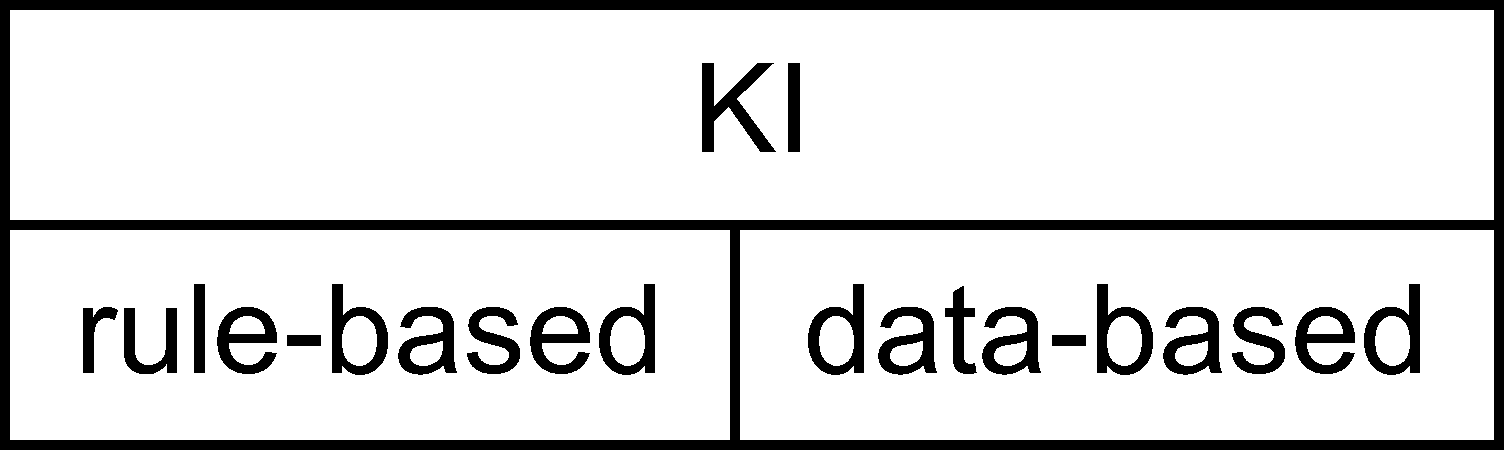
\includegraphics[width=0.5\linewidth]{chunk-img/ai-ml2-1}

In beiden Fällen finden Algorithmen Verwendung.
Algorithmen sind nichts anderes als genaue Schritt-für-Schritt-Anleitungen, um etwas zu erledigen.
Ein Kochrezept ist ein klassisches Beispiel für einen Algorithmus.

\href{https://www.c-programming-simple-steps.com/images/xsum-two-numbers-h.png.pagespeed.ic.AM9WYFPgEo.webp}{Hier} findet sich ein Beispiel für einen einfachen Additionsalgorithmus.

\hypertarget{rule-based}{%
\subsection{Rule-based}\label{rule-based}}

Klassische (ältere) KI implementiert Regeln ``hartverdrahtet'' in ein Computersystem.
Nutzer füttern Daten in dieses System. Das System leitet dann daraus Antworten ab.

\emph{Regeln} kann man prototypisch mit \emph{Wenn-Dann-Abfragen} darstellen:

\begin{verbatim}
## [1] "Durchgefallen!"
## [1] "Durchgefallen!"
## [1] "bestanden!"
## [1] "bestanden!"
\end{verbatim}

Sicherlich könnte man das schlauer programmieren, vielleicht so:

\begin{verbatim}
## # A tibble: 4 x 3
##   lernzeit schlauer_nebensitzer bestanden
##      <dbl> <lgl>                <lgl>    
## 1        0 FALSE                FALSE    
## 2       10 FALSE                FALSE    
## 3       10 TRUE                 TRUE     
## 4       20 TRUE                 TRUE
\end{verbatim}

\hypertarget{data-based}{%
\subsection{Data-based}\label{data-based}}

ML hat zum Ziel, Regeln aus den Daten zu lernen. Man füttert Daten und Antworten in das System, das System gibt Regeln zurück.

\citet{james_introduction_2021} definieren ML so:
Nehmen wir an, wir haben die abhängige Variable \(Y\) und \(p\) Prädiktoren, \(X_1,X_2, \ldots, X_p\).
Weiter nehmen wir an, die Beziehung zwischen \(Y\) und \(X = (X_1, X_2, \ldots, X_p)\) kann durch eine Funktion \(f\) beschrieben werden.
Das kann man so darstellen:

\[Y = f(X) + \epsilon\]

ML kann man auffassen als eine Menge an Verfahren, um \(f\) zu schätzen.

Anders gesagt: traditionelle KI-Systeme werden mit Daten und Regeln gefüttert und liefern Antworten.
ML-Systeme werden mit Daten und Antworten gefüttert und liefern Regeln zurück, vgl. Abb. \ref{fig:ki-ml2}.

\textbackslash begin\{figure\}{[}H{]}

\{\centering 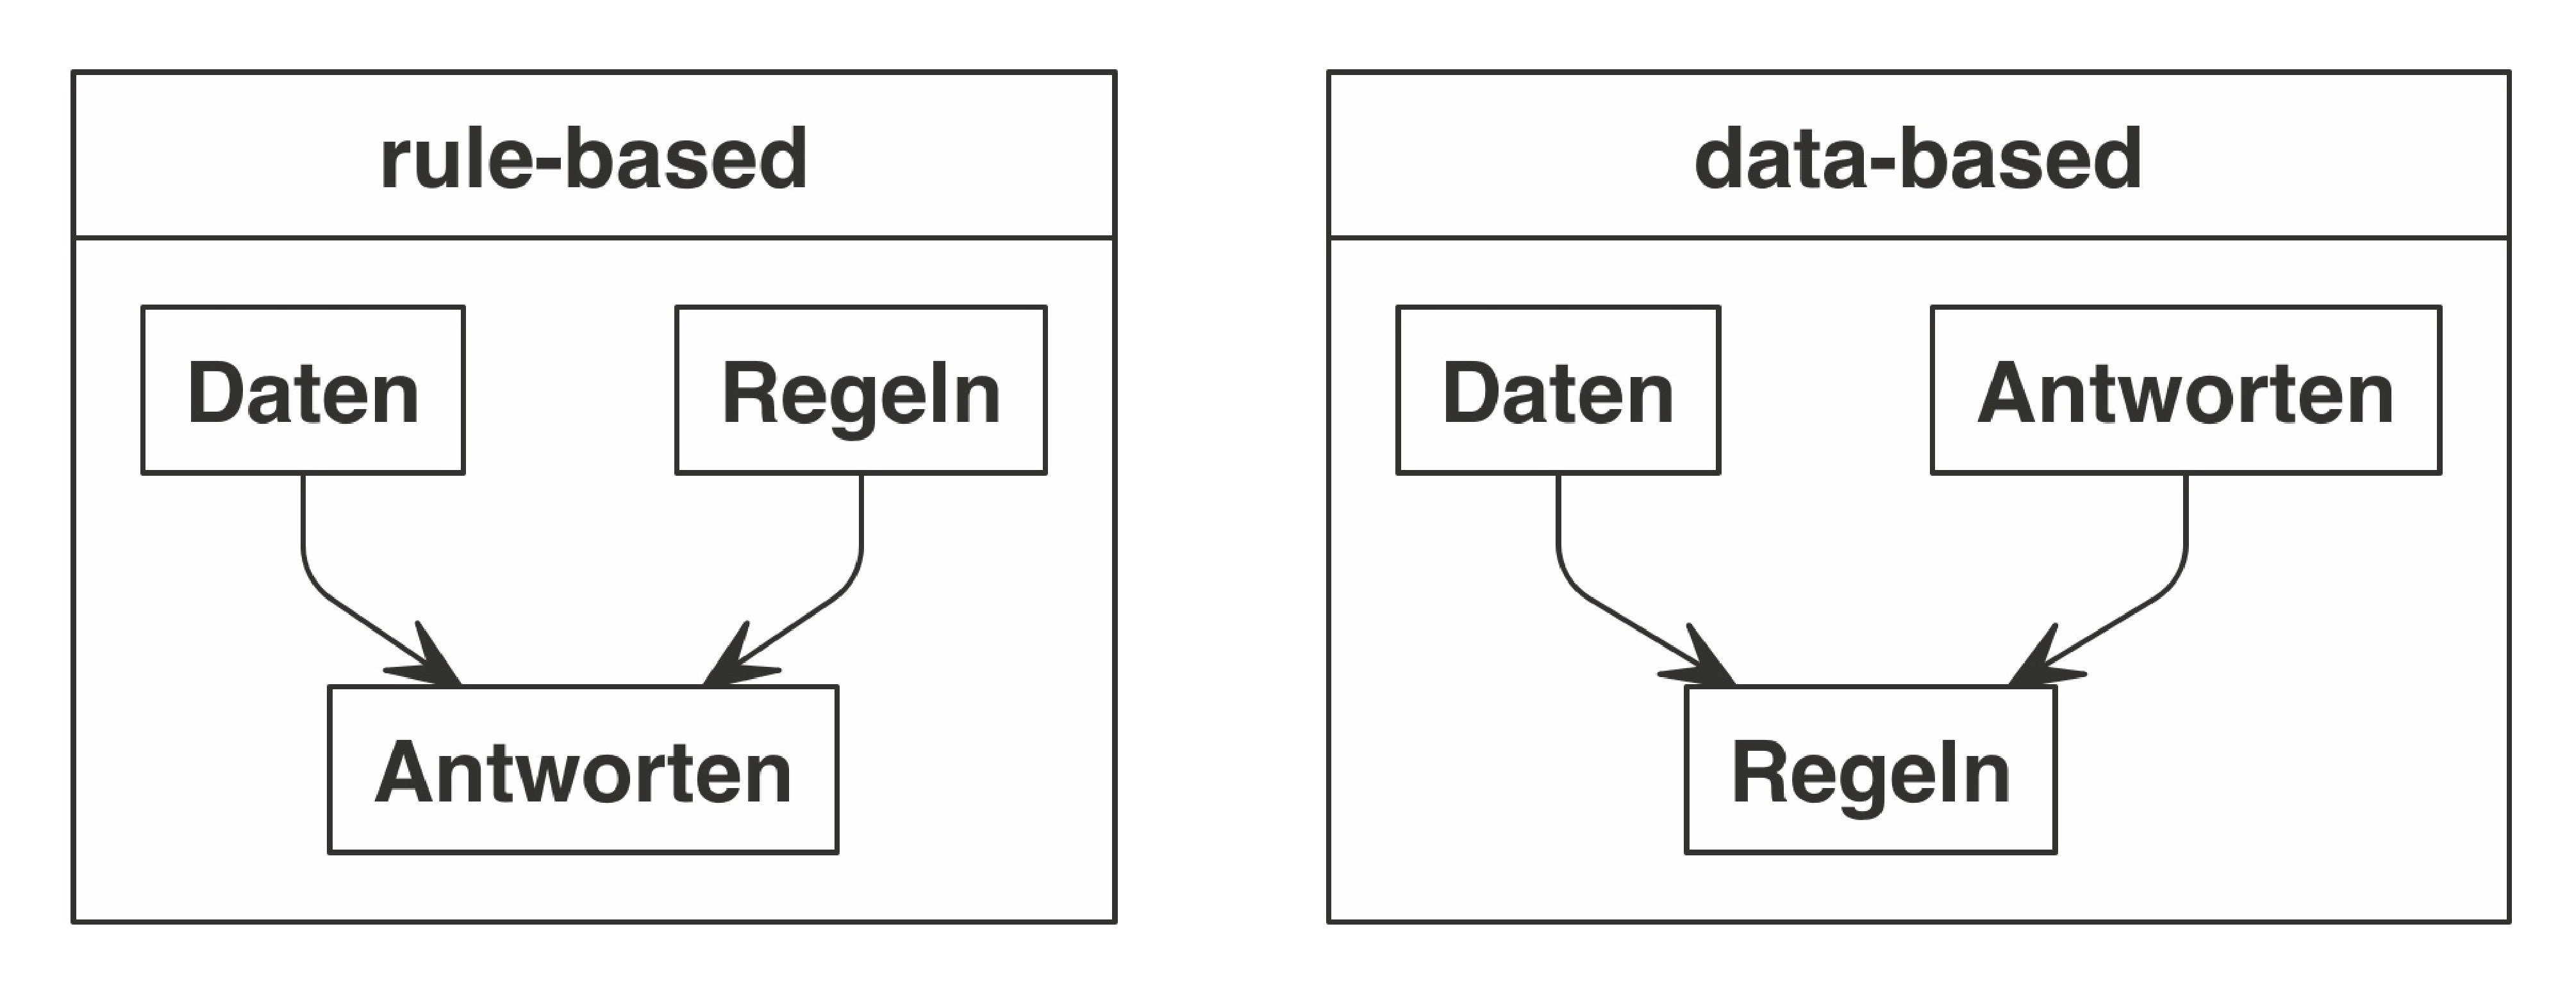
\includegraphics[width=0.5\linewidth]{chunk-img/ki-ml2-1}

\hypertarget{modell-vs.-algorithmus}{%
\section{Modell vs.~Algorithmus}\label{modell-vs.-algorithmus}}

\hypertarget{modell}{%
\subsection{Modell}\label{modell}}

Ein Modell, s. Abb. \ref{fig:vw} \citep{spurzem_vw_2017}!

\begin{figure}[H]

{\centering 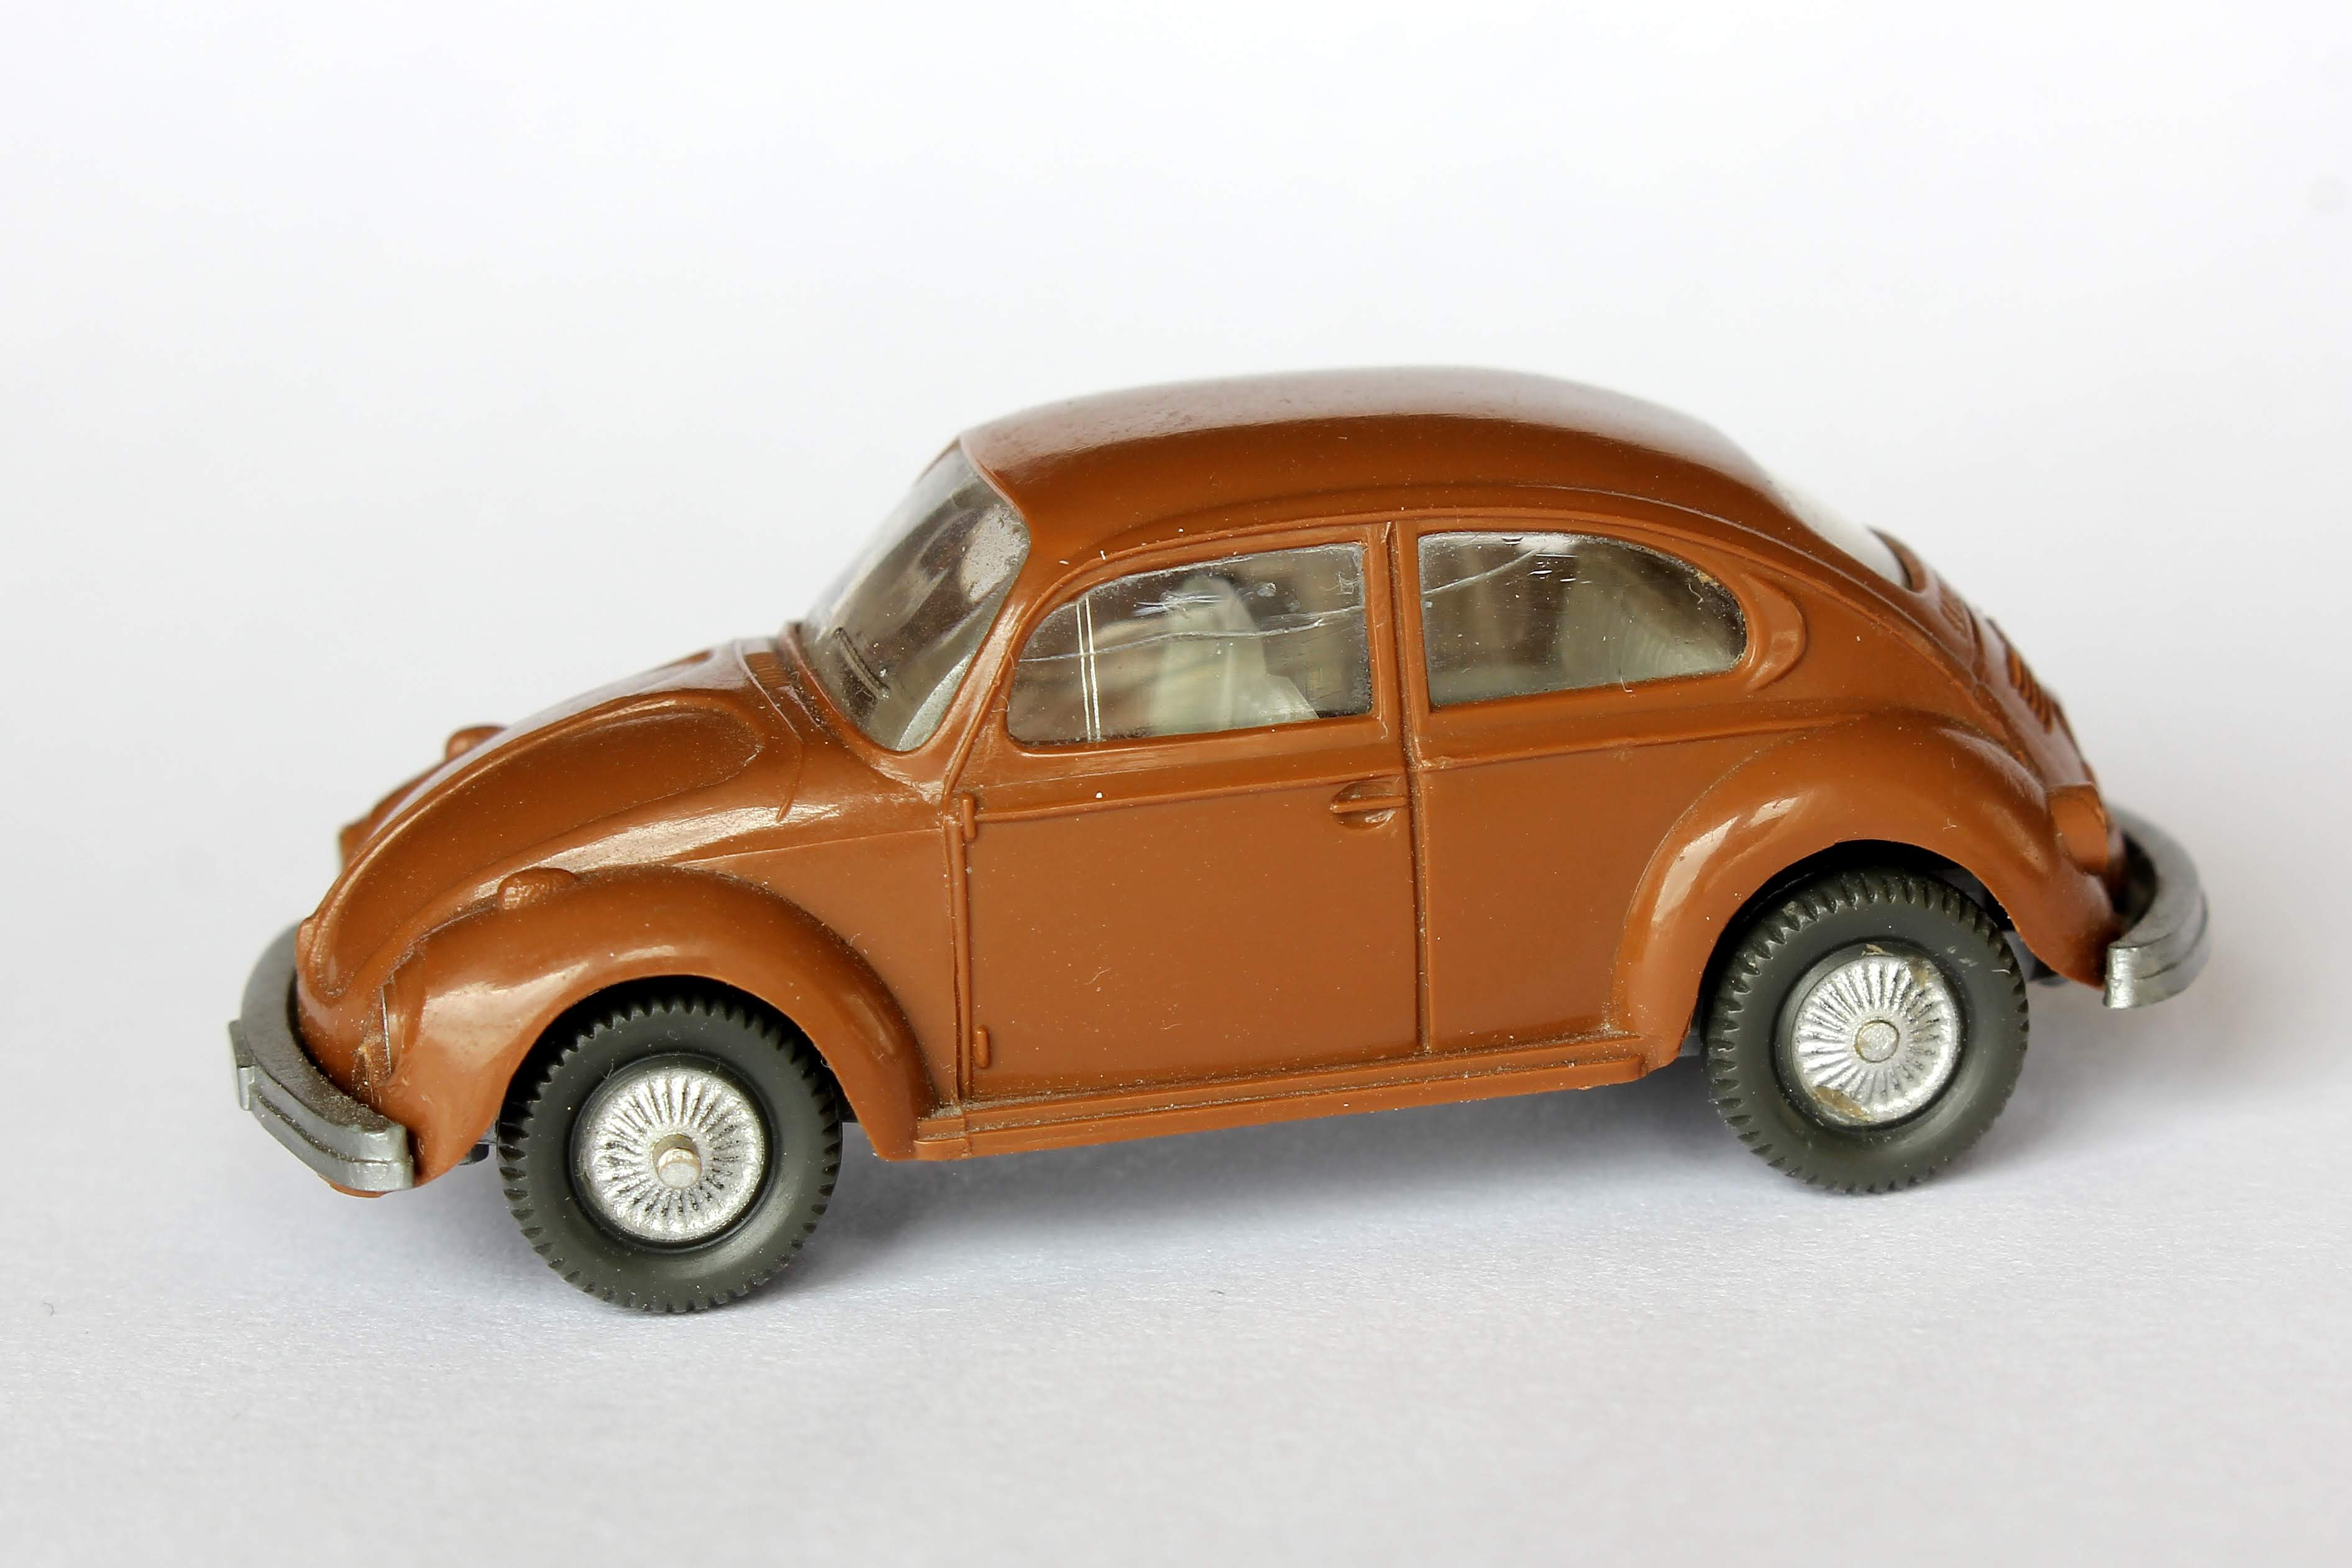
\includegraphics[width=0.33\linewidth]{img/vw_modell} 

}

\caption{Ein Modell-Auto}\label{fig:vw}
\end{figure}

Wie man sieht, ist ein Modell eine vereinfachte Repräsentation eines Gegenstands.

Der Gegenstand definiert (gestaltet) das Modell. Das Modell ist eine Vereinfachung des Gegenstands, vgl. Abb. \ref{fig:modell}.

\begin{figure}[H]

{\centering \includegraphics[width=0.5\linewidth]{img/modell-crop} 

}

\caption{Gegenstand und Modell}\label{fig:modell}
\end{figure}

Im maschinellen Lernen meint ein Modell, praktisch gesehen, die Regeln,
die aus den Daten gelernt wurden.

\hypertarget{beispiel-fuxfcr-einen-ml-algorithmus}{%
\subsection{Beispiel für einen ML-Algorithmus}\label{beispiel-fuxfcr-einen-ml-algorithmus}}

Unter einem ML-Algorithmus versteht man das (mathematische oder statistische) Verfahren,
anhand dessen die Beziehung zwischen \(X\) und \(Y\) ``gelernt'' wird. Bei \citet{rhys} (S. 9) findet sich dazu ein Beispiel, das kurz zusammengefasst etwa so lautet:

\emph{Beispiel eines Regressionsalgorithmus}

\begin{enumerate}
\def\labelenumi{\arabic{enumi}.}
\tightlist
\item
  Setze Gerade in die Daten mit \(b_0 = \hat{y}, b_1 = 0\)
\item
  Berechne \(MSS = \sum (y_i - \hat{y_i})^2\)
\item
  ``Drehe'' die Gerade ein bisschen, d.h. erhöhe \(b_1^{neu} = b_1^{alt} + 0.1\)
\item
  Wiederhole 2-3 solange, bis \(MSS < \text{Zielwert}\)
\end{enumerate}

Diesen Algorithmus kann man ``von Hand'' z.B. mit \href{https://shinyapps.org/showapp.php?app=https://shiny.psy.lmu.de/felix/lmfit\&by=Felix\%20Sch\%C3\%B6nbrodt\&title=Find-a-fit!\&shorttitle=Find-a-fit!}{dieser App} durchspielen.

\hypertarget{taxonomie}{%
\section{Taxonomie}\label{taxonomie}}

Methoden des maschinellen Lernens lassen sich verschiedentlich gliedern.
Eine typische Gliederung unterscheidet in \emph{supervidierte} (geleitete) und \emph{nicht-supervidierte} (ungeleitete) Algorithmen, s. Abb. \ref{fig:taxonomie}.

\textbackslash begin\{figure\}{[}H{]}

\{\centering 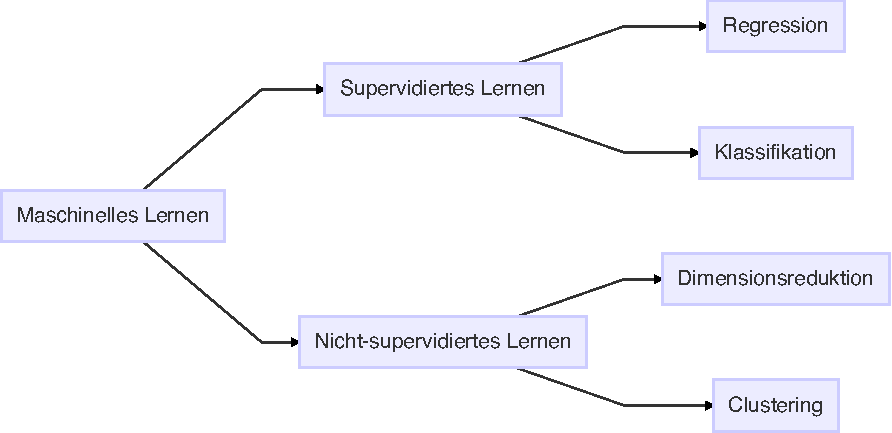
\includegraphics[width=0.5\linewidth]{chunk-img/taxonomie-1}

\hypertarget{ziele-des-ml}{%
\section{Ziele des ML}\label{ziele-des-ml}}

Man kann vier Ziele des ML unterscheiden, s. Abb. \ref{fig:ziele}.

\textbackslash begin\{figure\}{[}H{]}

\{\centering 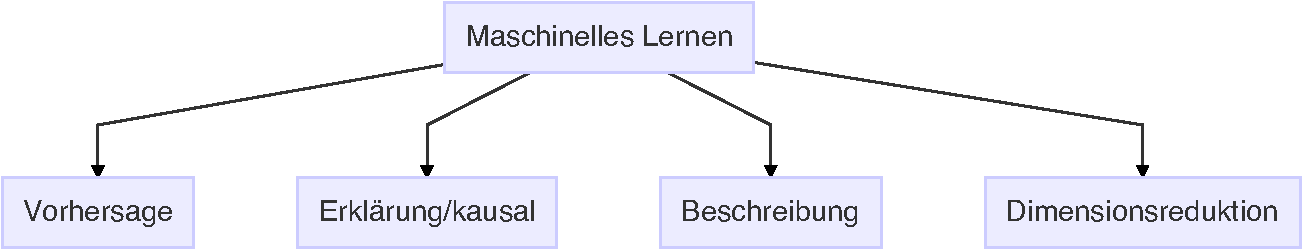
\includegraphics[width=0.5\linewidth]{chunk-img/ziele-1}

\emph{Vorhersage} bezieht sich auf die Schätzung der Werte von Zielvariablen (sowie die damit verbundene Unsicherheit).
\emph{Erklärung} meint die kausale Analyse von Zusammenhängen.
\emph{Beschreibung} ist praktisch gleichzusetzen mit der Verwendung von deskriptiven Statistiken.
\emph{Dimensionsreduktion} ist ein Oberbegriff für Verfahren, die die Anzahl der Variablen (Spalten) oder der Beobachtungen (Zeilen) verringert.s

\hypertarget{test}{%
\section{Test}\label{test}}

jköjk \ref{fig:test}

\textbackslash begin\{figure\}{[}H{]}

\{\centering 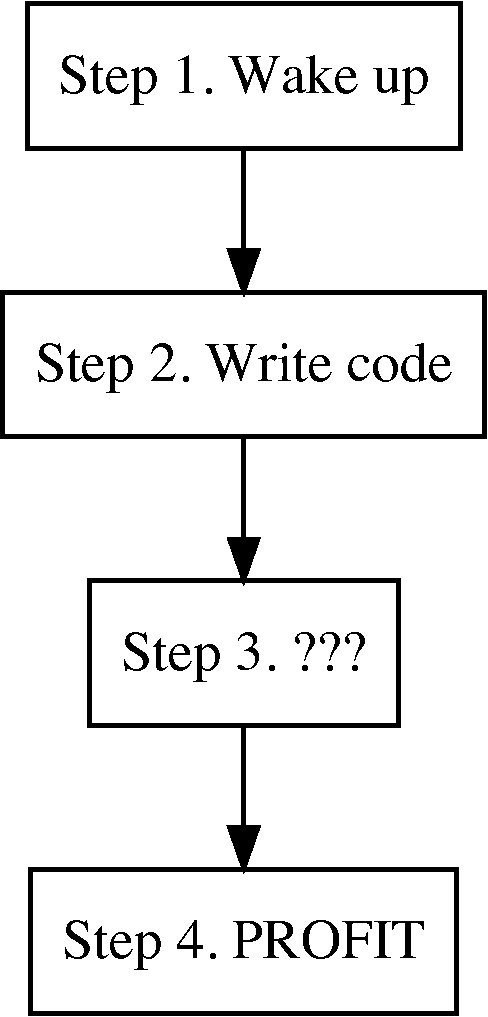
\includegraphics[width=0.5\linewidth]{chunk-img/test-1}

  \bibliography{book.bib,packages.bib}

\end{document}
